%%%%%%%%%%%%%%%%%%%%%%%%%%%%%%%%%%%%%%%%%%%%%%%%%%%%%%%%%%%%%%%%%
% Qualificacao de Doutorado / Dept Fisica, CFM, UFSC            %
% Eduardo@UFSC - 2015                                           %
%%%%%%%%%%%%%%%%%%%%%%%%%%%%%%%%%%%%%%%%%%%%%%%%%%%%%%%%%%%%%%%%%


%:::::::::::::::::::::::::::::::::::::::::::::::::::::::::::::::%
%                                                               %
%                          Capítulo 6                           %
%                                                               %
%:::::::::::::::::::::::::::::::::::::::::::::::::::::::::::::::%

%***************************************************************%
%                                                               %
%                      Conversão tauV - Gas                     %
%                                                               %
%***************************************************************%

\chapter{Estimando frações de gás}
\label{sec:gasfrac}

A fração de gás no modelo simples de evolução química ({\em closed-box model}) escala linearmente
com a metalicidade do gás, onde a inclinação da reta é o {\em yield}, que representa o quanto de
metais está sendo produzido e ejetado a cada geração de estrelas. Durante a pesquisa que nos levou a
escrever o artigo que está no Apênd. \label{apendice:GDetal2014b} encontramos uma relação
interessante que serviu de pontapé inicial para todo esse nosso projeto. Nesse capítulo vamos
comentar brevemente sobre nosso progresso nessa conversão para nossas galáxias e discutir quais os
desafios enfrentados até agora e aqueles que estão por vir nas próximas estapas de nosso projeto.

\section{Um modelo simples de evolução química}
\label{sec:gasfrac:closedbox}

A relação da qual comentamos no preambulo deste capítulo pode ser vista na Fig.
\ref{fig:dust2stars}. A razão entre o coeficiente de extinção e a densidade superficial de massa
estelar ($A_V / \mu_\star$) parece relacionar de maneira interessante com a metalicidade média das
populações estelares e nos motivou a buscar a conversão de poeira em gás e poder compará-la com a
metalicidade nebular.
\begin{figure}
	\centering
	%\resizebox{0.7\textwidth}{!}{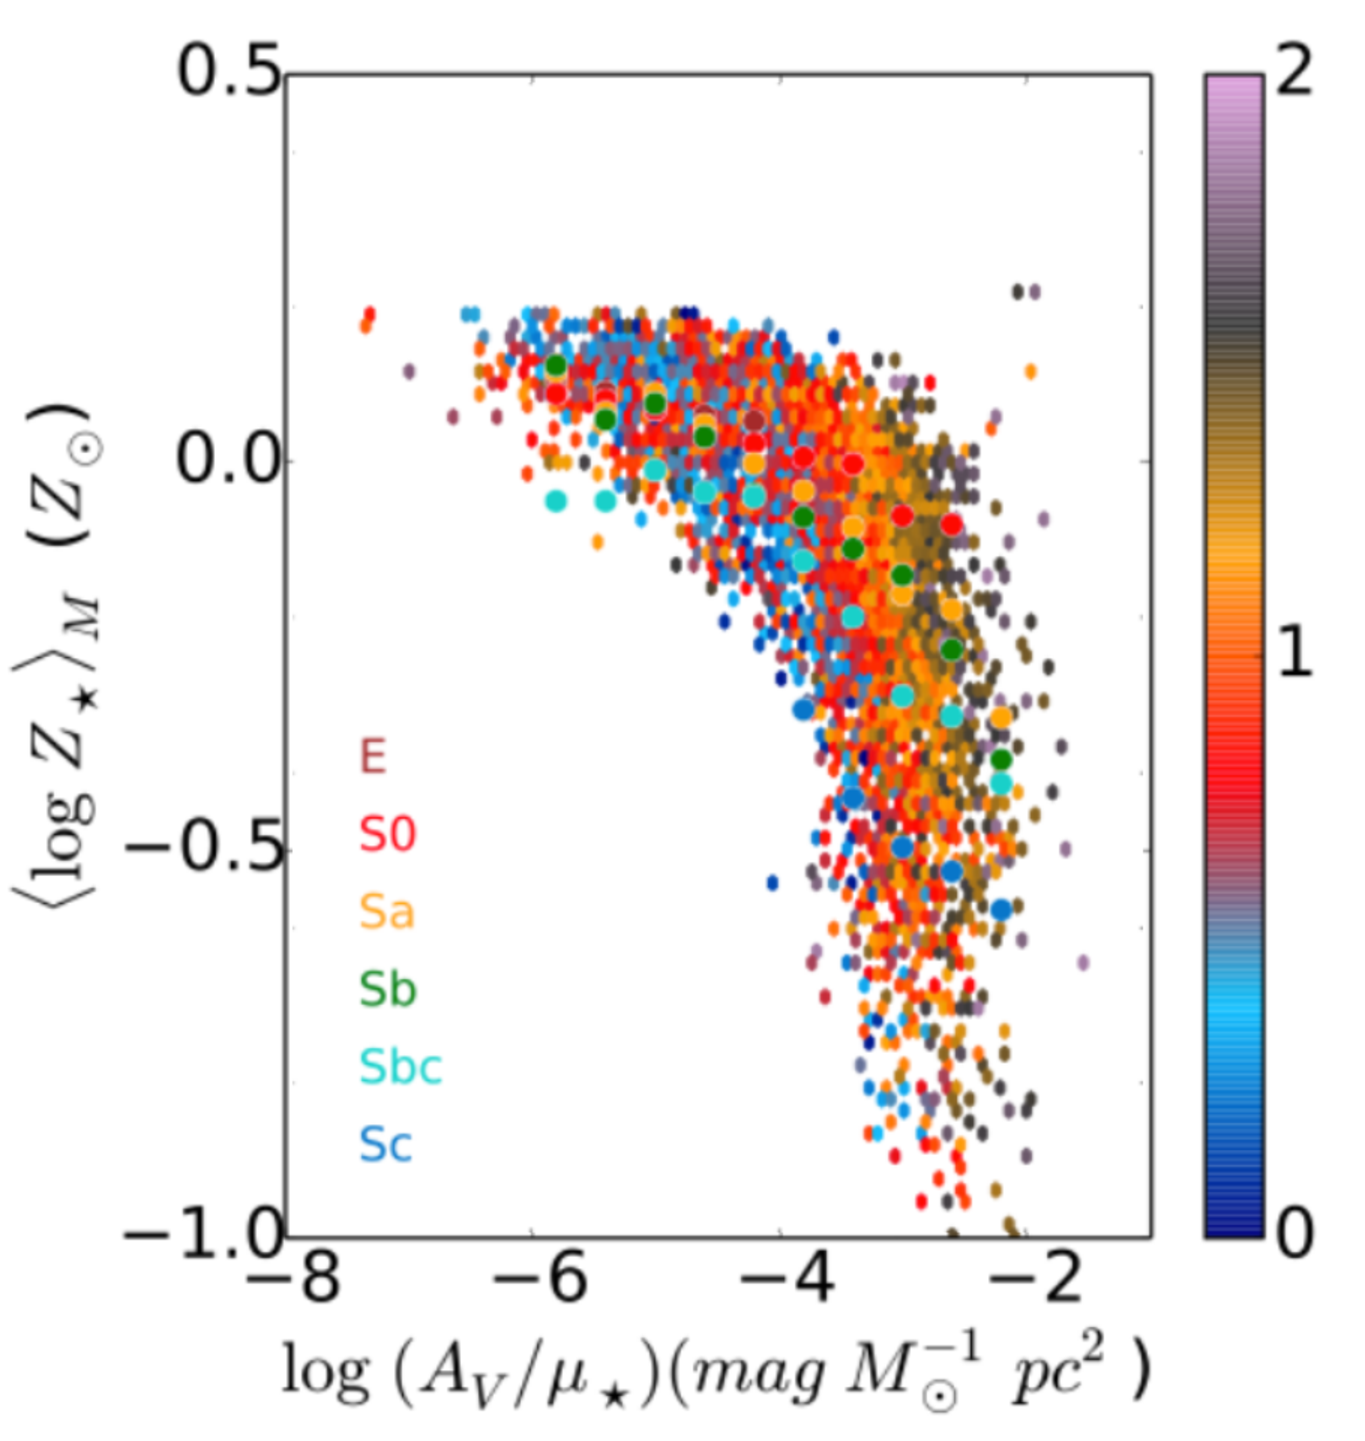
\includegraphics{figuras/dust2stars.pdf}}
	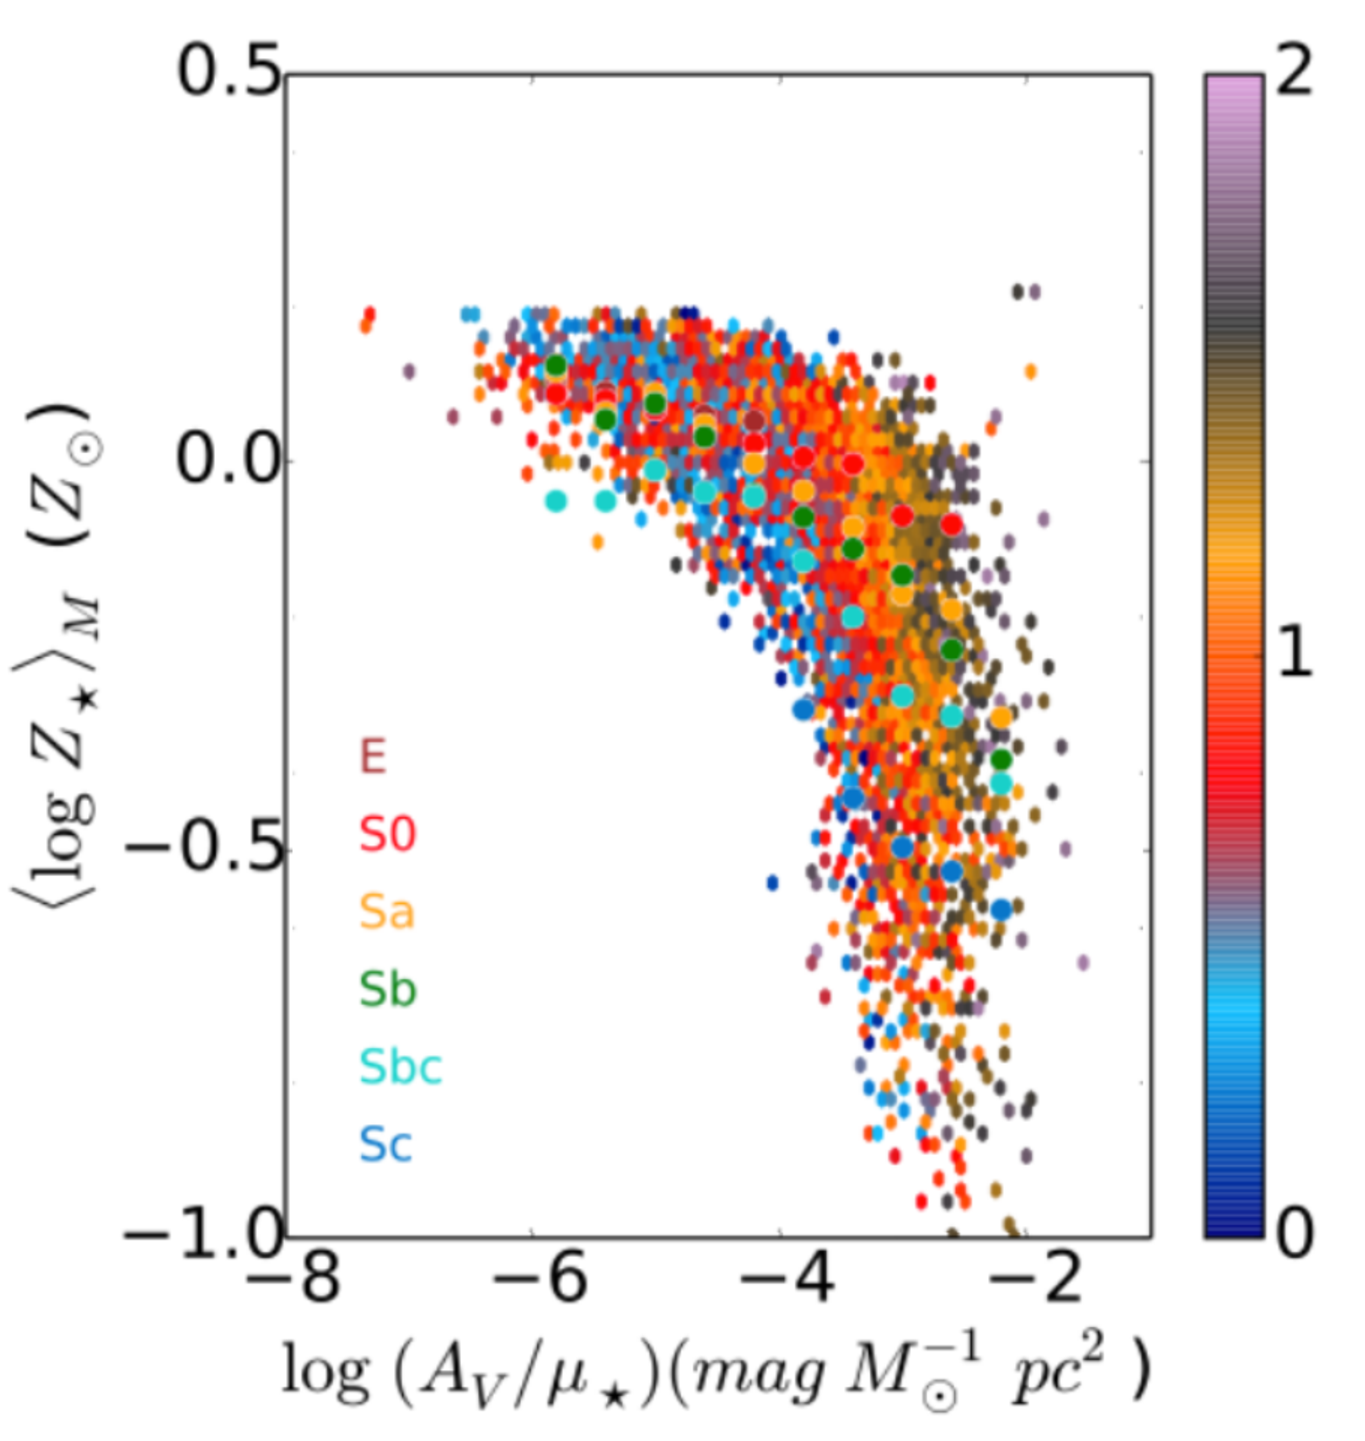
\includegraphics[height = 8cm, width = 9.5cm]{figuras/dust2stars.pdf}
	\caption[$A_V / \mu_\star$ vs. \meanM{\log Z_\stars}]
	{Relação entre metalicidade média das populações estelares e a razão entre o coeficiente de
extinção (em magnitude) e a densidade superficial de massa estelar. Os pontos estão divididos em
cores por tipo morfológico.}
	\label{fig:dust2stars}
\end{figure}
O principal objetivo de nosso trabalho é pode estimar fração de gás espacialmente resolvidas nas
galáxias do CALIFA. Podemos definir fração de gás como:
\begin{equation}
	f_{\mathrm{gas}} = \frac{\mathrm{M}_{\mathrm{gas}}}{\mathrm{M}_\star + \mathrm{M}_{\mathrm{gas}}}
\equiv \frac{1}{1 + \frac{\mathrm{M}_\star}{\mathrm{M}_{\mathrm{gas}}}},
	\label{eq:fgas}
\end{equation}
\noindent onde $M_{\mathrm{gas}}$ é a massa total na forma de gás e $M_\star$ é a massa total em
estrelas. 

Em um modelo simples de evolução química de uma galáxia onde não exista nem {\em inflow} nem {\em
outflow} de gás, isto é, uma galáxia isolada em um sistema fechado sem entrada de mais gás além do
inicial e nem perda, a metalicidade do gás pode ser escrita como:
%\begin{eqnarray}
%	Z_{\mathrm{gas}} &=& y \ln \left(1/f_{\mathrm{gas}}\right) \\
%	\label{eq:Zgas_closedbox}
%	\langle Z_\star \rangle_M &=& y \left(1 - \frac{f_{\mathrm{gas}} \ln (1/f_{\mathrm{gas})}}{1 -
%	f_{\mathrm{gas}}} \right)
%	\label{eq:Zstar_closedbox}
%\end{eqnarray}
\begin{equation}
	Z_{\mathrm{gas}} = - y \ln f_{\mathrm{gas}},
	\label{eq:Zgas_closedbox}
\end{equation}
\noindent onde $y$ é o {\em yield}. Essa primeira equação foi derivada explicitamente pela primeira
vez por \citet{Searle.Sargent.1972a} ao estudar duas regiões \Hii gigantes, ditas ``isoladas''.
Nesse cenário, o {\em yield} e pode ser aproximado quando conhecemos $Z_{\mathrm{gas}}$ e
$f_{\mathrm{gas}}$.

\section{Relação de Kennicut-Schmidt e nossa {\em pseudo-KS}}
\label{sec:gasfrac:KS}

Como explicado na Sec. \ref{sec:intro:galaxias}, a quantidade de gás de uma galáxia e a taxa de
formação estelar parecem estar relacionadas através de uma lei de potências. Pensando nisso,
estabelecemos nossa relação entre poeira e formação estelar, que pode ser vista na Fig.
\ref{fig:pseudoKS}. No painel esquerdo usamos $\tauVS$ como nossa variável representante da poeira e
no direito, $\tauVN$. A conversão de poeira em gás é, da mesma forma que a conversão de CO em gás,
dependente da metalicidade, mas com a vantagem de não necessitar medidas. O espalhamento nesta
figura nos mostra que podemos explorar os resíduos em torno desse ajuste.

\begin{figure}
	\centering
	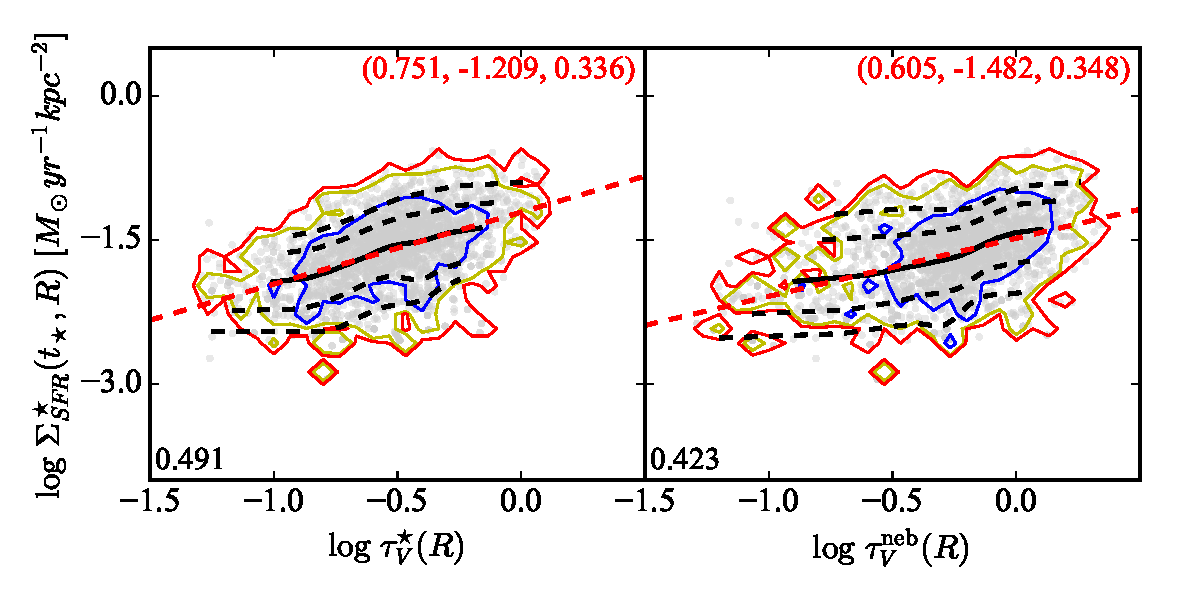
\includegraphics[width=0.95\textwidth]{figuras/pseudoKS.pdf}
	\caption[Nossa {\em pseudo-KS}.]
	{Relação entre a densidade superficial da taxa de formação estelar e o coeficiente de extinção
proveniente da síntese ($\tauVS$ - {\em painel esquerdo}) e do decremento de Balmer ($\tauVN$ -
{\em painel direito}). A linha tracejada em vermelho marca o ajuste linear da mediana e os
valores marcam o coeficiente de correlação de Spearmann (canto inferior esquerdo) e a
inclinação, valor de interceptação do eixo y e o valor do desvio médio quadrático da distribuição em
torno do ajuste (canto superior direito).}
	\label{fig:pseudoKS}
\end{figure}

\subsection{Resíduos da pseudo-KS}
\label{sec:gasfrac:KS:resid}
 
Na Fig. \ref{fig:pseudoKSresid} podemos ver \ldots 
\begin{figure}
	\centering
	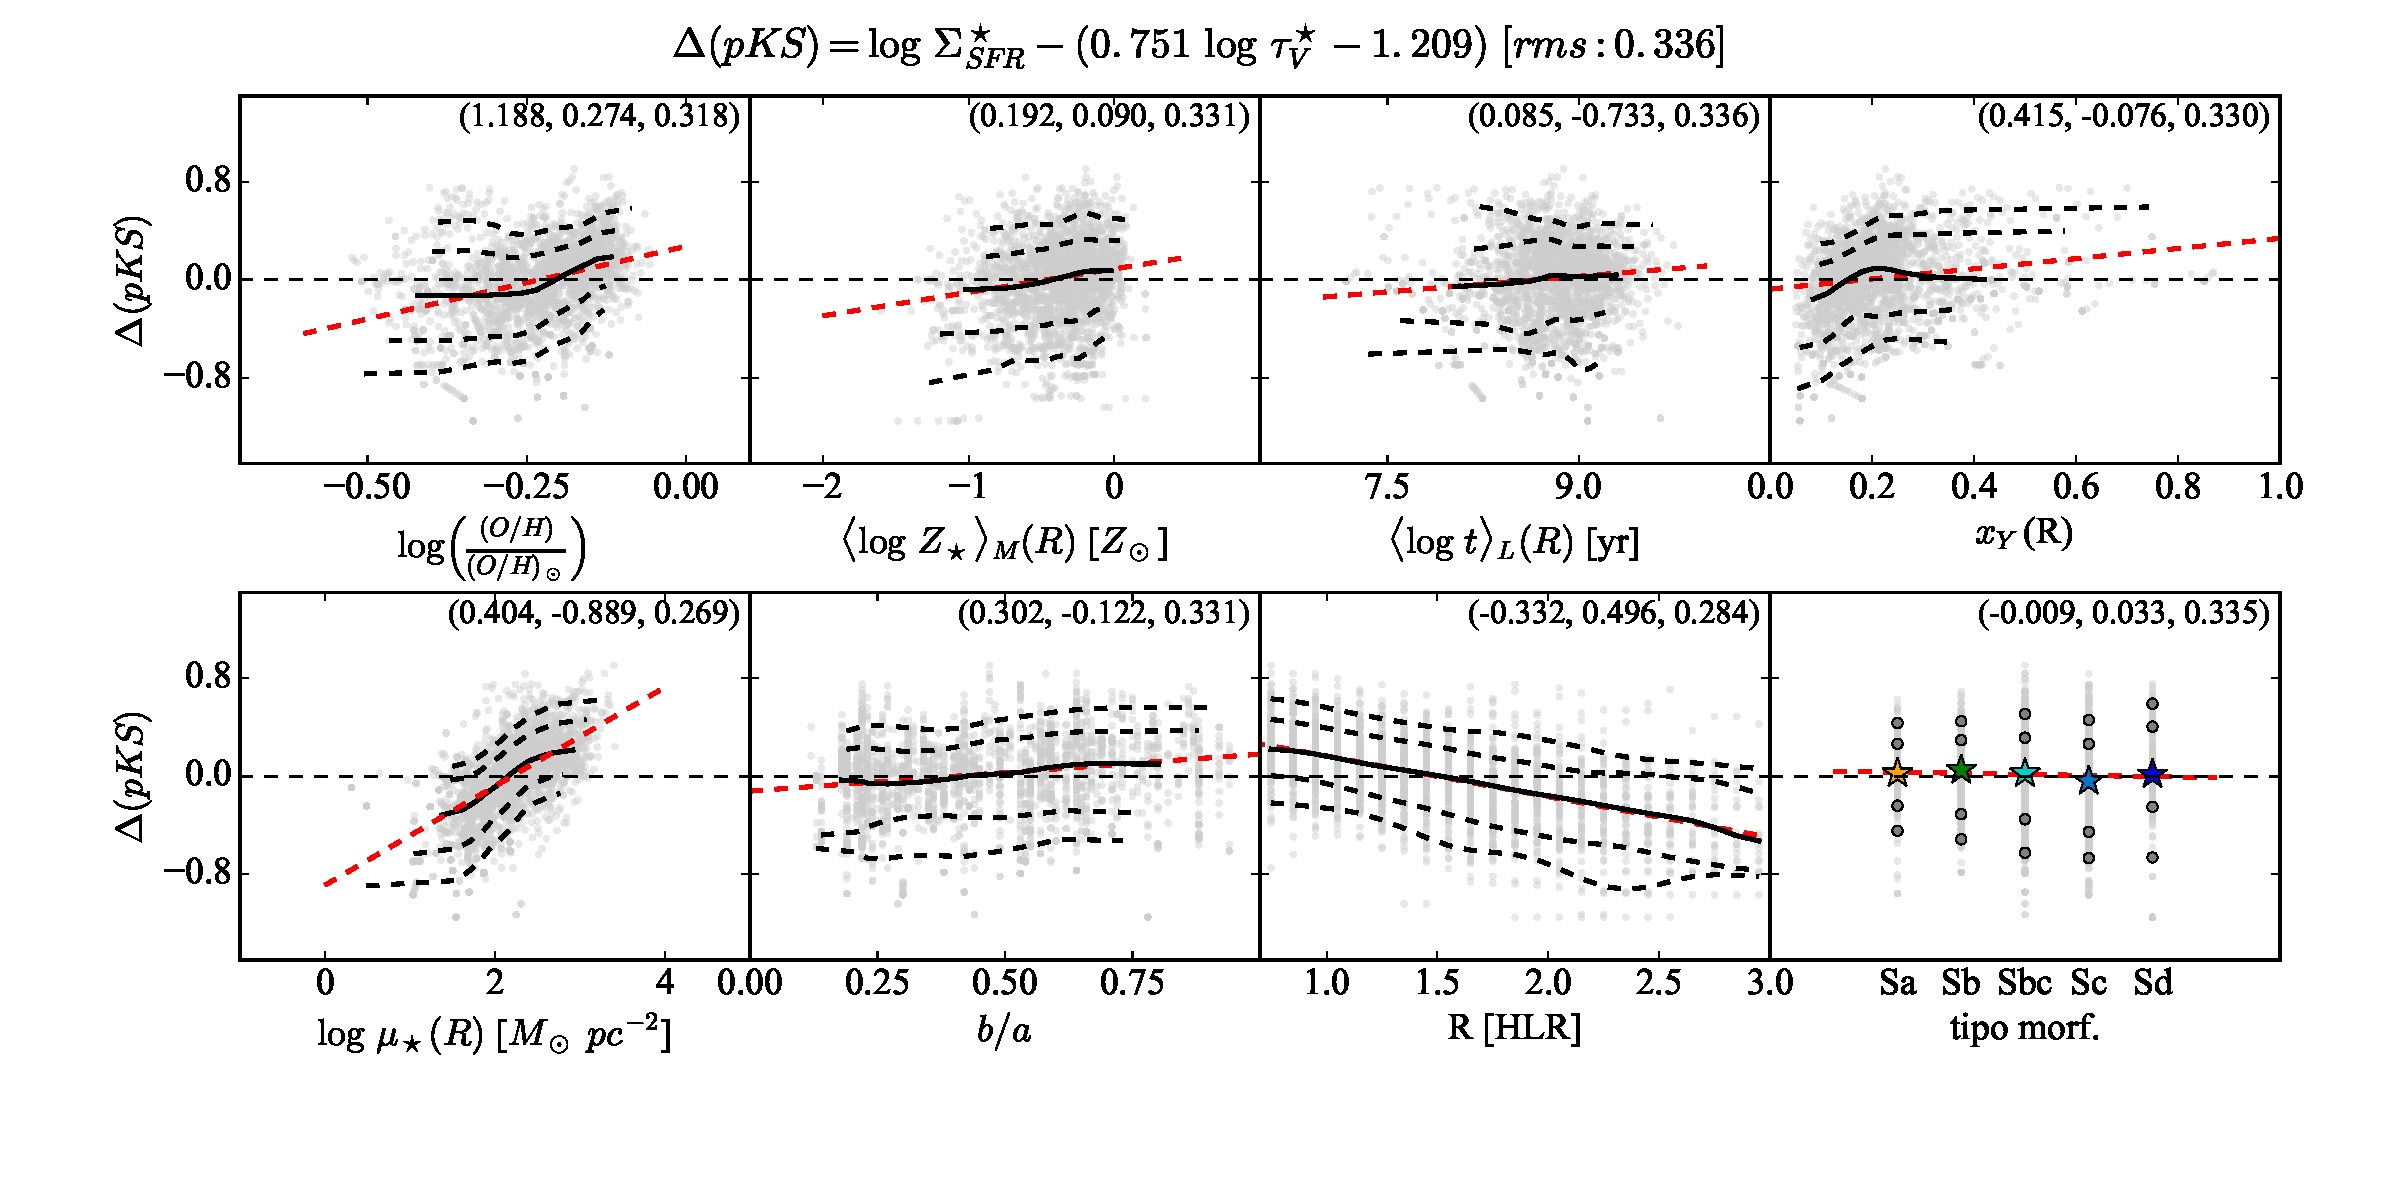
\includegraphics[width=0.99\textwidth]{figuras/deltapKS.pdf}
	\caption[Resíduos da {\em pseudo-KS}.]
	{No eixo y de todos os painés temos $\Delta_{pKS} = \SimgaSFR - (0.791 \tauVS - 1.191)$, onde, o
termo entre parenteses é o ajuste linear da mediana no painel esquerdo da Fig. \ref{fig:pseudoKS}.
No eixo x temos, na primeira fila, da esquerda para direita: metalicidade nebular ($12 + \log
(O/H)$), metalicidade estelar média pesada pela massa ($\meanM{\log Z_\star}$), idade média das
populações estelares ($\meanL{\log t_\star}$), fração em luz das populações estelares jovens
($x_Y$); na última fila, na mesma ordem: densidade superficial de massa estelar, relação axial, raio
e tipo morfológico.}
	\label{fig:pseudoKS}
\end{figure}

Diversos autores atualmente calculam e discutem a relação KS e a sua validade para diferentes
resoluções espaciais \citep[e.g., ][]{Kennicutt.etal.2007a, Leroy.etal.2012a,
Calzetti.Liu.Koda.2012a, Lada.etal.2013a, Tacconi.etal.2013a, Casasola.etal.2015a}. A inclinação
da KS (N = 1.4 na Eq. \ref{eq:SFRKennicutt}) varia geralmente entre 1 e 2, dependendo da resolução
espacial observada (regiões \Hii, perfis radiais, galáxias integradas) ou do tipo de gás usado
(atômico, molecular ou a soma dos dois).

\section{Conversão de poeira em gás.}
\label{sec:gasfrac:gas2dust}

Para converter poeira em gás primeiro precisamos da densidade superficial de poeira, que pode ser
conseguida utilizando a equação:
\begin{eqnarray}
	\tau_{\mathrm{d}} &=& \sigma_{\mathrm{d}} \int n_{\mathrm{d}} dz =
	\frac{\sigma_{\mathrm{d}}}{m_{\mathrm{d}}}\times\Sigma_{\mathrm{d}}
	\\
	\Sigma_{\mathrm{d}} &=& \frac{m_{\mathrm{d}} \tau_{\mathrm{d}}}{\sigma_{\mathrm{d}}},
	\label{eq:sigmadust}
\end{eqnarray}
\noindent onde o prefixo d designa poeira ({\em dust}, em inglês), $\sigma_{\mathrm{d}}$ é área de
um grão de poeira, $n_{\mathrm{d}}$ é o número de grãos de poeira ao longo de uma profundidade
$dz$ e $m_{\mathrm{d}}$ é a massa de um grão de poeira. Substituindo a Eq. \ref{eq:sigmadust} na Eq. 
\ref{eq:dust2gas} e assumindo $\tauV$ como $\tau_{\mathrm{d}}$ obtemos:
\begin{equation}
	\SigmaGas\ =\ \frac{m_{\mathrm{d}}}{\sigma_{\mathrm{d}}}\ \deltaDGR\ \tauV. 
	\label{eq:dust2gas_tauV}
\end{equation}
O termo $\deltaDGR$ é dependente da metalicidade e vamos explorar a conversão feita por
\citet{Brinchmann.etal.2013a}. Neste trabalho os autores seguem o modelo de absorção de
\ref{Charlot.Fall.2000a} e identificam algumas variáveis que vamos utilizar:
\begin{eqnarray}
	\xi &=& \frac{\Sigma_{\mathrm{d}}}{\Sigma_Z} \\
	Z &=& \frac{\Sigma_Z}{\SigmaGas}  \\
	\delta_{\mathrm{DGR}} &=& \frac{\Sigma_{\mathrm{d}}}{\SigmaGas} = \xi Z, 
	\label{eq:deltaDGR}
\end{eqnarray}
\noindent onde $\xi$ é a razão poeira-metais ({\em dust-to-metals}) e Z é a metalicidade do gás.
Utilizando a Eq. \ref{eq:deltaDGR} na Eq. \ref{eq:dust2gas_tauV} e fazendo
$m_{\mathrm{d}}/\sigma_{\mathrm{d}} \approx 0.2$, que corresponde ao tipo de poeira Galáctica, temos:
\begin{equation}
	\SigmaGas\ \approx\ 0.2 \frac{\tauV}{\delta_{\mathrm{DGR}}}\ [M_\odot pc^{-2}].
	\label{eq:dust2gas_brinch}
\end{equation}
Neste artigo os autores utilizaram dados de $\sim 70000$ galáxias {\em star-forming} do
\textit{SDSS}-DR7 e parametrizam $\delta_{\mathrm{DGR}}$ como \citep[][Eq.
28]{Brinchmann.etal.2013a}:
\begin{equation}
	\delta_{\mathrm{DGR}}\ =\ (5.3 \times 10^{-3} - 1.1 \times 10^{-2})
\left(\frac{\mathrm{O/H}}{(\mathrm{O/H})_\odot}\right),
	\label{eq:DGR_brinch_eq28}
\end{equation}
\noindent onde os fatores que multiplicam a metalicidade representam um intervalo onde esta
conversão é válida.

O valor de $\delta_{\mathrm{DGR}}$ foi parametrizado utilizando as metalicidades 

precisamos 
\ref{eq:DGR_brinch_eq28}

\section{Eficiência e tempo de depleção do gás.}
\label{sec:gasfrac:SFE}

Um outro tipo de abordagem é trabalhar com a eficiência da transformação de gás em estrelas,
utilizando a relação:
\begin{equation}
	\mathrm{SFE} = \frac{\Sigma_{\mathrm{SFR}}}{\Sigma_{\mathrm{gas}}} = \frac{1}{t_{\mathrm{dep}}},
	\label{eq:SFE}
\end{equation}
\noindent onde SFE vem de {\em star-formation efficiency} e $t_{\mathrm{dep}}$, que é o inverso da
eficiência, é o tempo de depleção do gás, que nos dá uma ideia da escala de tempo em que a galáxia
consome todo o gás com a taxa em que está formando estrelas.

\ldots
%\chapter{Coeficiente de extinção como indicador de Gás}
%\label{sec:gas}
% Referências:
% - Brinchman
% - Guiderdoni & Rocca
% - procurar mais conversões dust to gas ou dust to stars
% - Referências para cada indicador
%\section{Indicadores de gás}
%\label{sec:synvsneb:proxies}
% Figuras:
% - ?? retiradas alguns papers para diferentes indicadores ??
%\section{Lei de Schimidt-Kennict}
%\label{sec:synvsneb:proxies}
% Figuras:
% - sample SK
% - our pseudo - SK
%\section{De poeira para gás}
%\label{sec:synvsneb:proxies}
% Figuras:
% - perfis radiais de SigmaGas e de fgas
% - real SK

% End of this chapter
